\noindent\makebox[\linewidth][c]{学号：\underline{\hspace{9em}}\qquad 姓名：\underline{\hspace{9em}}}\par
\pdfbookmark[0]{一、填空题}{fillin}
\section{填空题（26 分）}
\begin{question}[index=1]
请写出以下问题是由哪一层协议解决的：（1）在 \underline{\hspace{4em}} 层决定数据报的路径；（2）在 \underline{\hspace{4em}} 层把传输的位流分成数据帧；（3）在 \underline{\hspace{4em}} 层将光脉冲变换为二进制码。
\end{question}
\begin{question}[index=2]
10Base-T 网卡接收到如图 1 所示信号波形，该网卡收到的比特串可能是（4）\underline{\hspace{7em}}。
\par\smallskip\noindent\makebox[\linewidth][c]{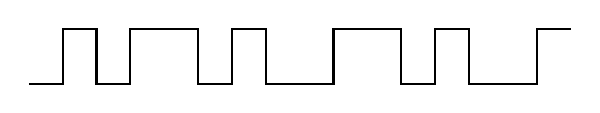
\begin{tikzpicture}[x=0.43cm,y=0.7cm]
\draw[line width=0.8pt] (0,0)--(1,0)--(1,1)--(2,1)--(2,0)--(3,0)--(3,1)--(5,1)--(5,0)--(6,0)--(6,1)--(7,1)--(7,0)--(9,0)--(9,1)--(11,1)--(11,0)--(12,0)--(12,1)--(13,1)--(13,0)--(15,0)--(15,1)--(16,1);
\end{tikzpicture}
}
\par\noindent\makebox[\linewidth][c]{图 1}
\end{question}
\begin{question}[index=3]
图 2 所示网络中，若主机 H 发送一个封装访问 Internet 的 IP 分组的 IEEE 802.11 数据帧 F，则帧 F 的地址 1、地址 2 和地址 3 分别是（5）\underline{\hspace{5em}}、（6）\underline{\hspace{5em}}、（7）\underline{\hspace{5em}}。
\par\smallskip\noindent\makebox[\linewidth][c]{\begin{tikzpicture}[x=1cm,y=1cm,every node/.style={inner sep=3pt}]
\node[draw,rectangle,minimum width=9mm,minimum height=7mm] (H) at (0,0) {H};
\node[draw,rectangle,minimum width=9mm,minimum height=9mm] (AP) at (4,0) {AP};
\node[draw,circle,minimum size=9mm] (R) at (8,0) {R};
\node[draw,cloud,cloud puffs=10,cloud puff arc=120,aspect=2,minimum width=2cm,minimum height=1cm] (I) at (10.5,0) {Internet};
\draw[dashed,->,line width=.6pt] (H)--(AP);
\node[draw,minimum width=8mm,minimum height=5mm] at (2,.5) {F};
\draw (AP)--(R)--(I);
\node[above] at (6,.1) {00-12-34-56-78-9c};
\node[below] at (0,-.55) {00-12-34-56-78-9a};
\node[below] at (4,-.55) {00-12-34-56-78-9b};
\end{tikzpicture}
}
\par\noindent\makebox[\linewidth][c]{图 2}
\end{question}
\begin{question}[index=4]
采用 CRC 校验，生成多项式为 $G(X)=X^4+X+1$（即 $G=10011$），则收到 101111000 时，可以断定在传输过程中（8）\underline{\hspace{4em}}（有或没有）发生错误。
\end{question}
\begin{question}[index=5]
奈奎斯特定理和香农定理是通信领域中的两个重要定理，它们分别描述了无噪声和有限噪声信道的最大数据传输速率。已知某通信链路带宽为 3kHz。在无噪声情况下，采用 4 个相位，每个相位具有 4 种振幅的 QAM 调制技术，则该通信链路的最大数据传输速率是（9）\underline{\hspace{5em}}。若信道信噪比为 30dB，则该链路的最大数据传输速率约为（10）\underline{\hspace{5em}}。
\end{question}
\begin{question}[index=6]
某网络的 IP 地址空间为 192.168.5.0/24，采用定长子网划分，子网掩码为 255.255.255.248，则该网络中的最大子网个数为（11）\underline{\hspace{2em}}，每个子网内的最大可分配地址个数分别是（12）\underline{\hspace{2em}}。
\end{question}
\begin{question}[index=7]
根据图 3 的路由表，目的地址为 128.9.25.9 的数据报应该送往（13）\underline{\hspace{5em}}。
\par\smallskip\noindent\makebox[\linewidth][c]{%
\begin{tabular}{|l|c|}\hline
Prefix & Port\\\hline
--- & ---\\\hline
128.9/16 & 5\\\hline
128.9.16/20 & 2\\\hline
128.9.19/24 & 7\\\hline
128.9.25/24 & 10\\\hline
128.9.176/20 & 1\\\hline
--- & ---\\\hline
\end{tabular}}
\par\noindent\makebox[\linewidth][c]{图 3（推定补全）}
\end{question}
\newpage
\pdfbookmark[0]{二、简答题}{short}
\section{简答题（29 分）}
\begin{question}[index=1]
（10 分）为什么要设计 IPv6？请比较 IPv6 和 IPv4 头部格式的差异。
\end{question}
\begin{question}[index=2]
（9 分）Traceroute 是一种常用的网络诊断工具，用于跟踪数据包从源主机到目标主机所经过的路径，并显示沿途所有路由器的 IP 地址和响应时间。请描述 Traceroute 的工作原理。
\end{question}
\begin{question}[index=3]
（10 分）CSMA/CD 协议和 CSMA/CA 协议分别是用来干什么的？它们的区别是什么？
\end{question}
\pdfbookmark[0]{三、计算题}{calculation}
\section{计算题（45 分）}
\begin{question}[index=1]
（9 分）假设一个采用 CSMA/CD 协议的 100Mbps 局域网，最小帧长是 128B，则在一个冲突域内两个站点之间的单向传播延时最多是多少？请给出分析和计算过程。
\end{question}
\begin{question}[index=2]
（20 分）已知网络拓扑如图 3 所示，请回答以下问题，并给出计算过程。
\par\smallskip\noindent\makebox[\linewidth][c]{\begin{tikzpicture}[x=1cm,y=1cm,every node/.style={inner sep=2pt}]
\node[draw,rectangle,minimum width=1cm,minimum height=.7cm] (A) at (0,0) {主机 A};
\node[draw,circle,minimum size=9mm] (R) at (6,0) {R};
\node[draw,rectangle,minimum width=1cm,minimum height=.7cm] (B) at (12,0) {主机 B};
\draw (A)--node[below]{链路 1}(R)--node[below]{链路 2}(B);
\node[align=center,above] at (3,.25) {10.2.128.1\\00-21-27-21-51-EE};
\node[align=center,above] at (9,.25) {101.12.123.15\\00-21-2E-1A-47-5B};
\node[below] at (6,-.65) {路由器 R};
\node[align=center,below] at (0,-.65) {IP：10.2.128.100\\MAC：00-15-C5-C1-5E-28};
\node[align=center,below] at (12,-.65) {IP：64.170.98.32\\MAC：00-68-AE-C2-37-FE};
\end{tikzpicture}
}
\par\noindent\makebox[\linewidth][c]{图 3}
\begin{enumerate}[label=\alph*)]
\item 主机 A 通过 1 个路由器 R（存储转发方式）与主机 B 互联，两段链路的数据传输速率均为 10Mbps。主机 A 分别采用报文交换和分组大小为 10kb 的分组交换向主机 B 发送 1 个大小为 8Mb（$1\mathrm{M}=10^6$）的报文。若忽略链路传播延迟、分组头开销和分组拆装时间，则两种交换方式完成该报文传输所需的总时间分别为多少？请写出计算过程。
\item 主机 A 向主机 B 发送数据，主机 A 在构造相关帧时，目的 MAC 地址是什么？如果主机 A 不知道目的 MAC 地址，使用什么协议确定目的 MAC 地址？封装该协议请求报文的以太网帧的目的 MAC 地址是什么？
\item 假设主机 A 向主机 B 发送一个总长度为 1500B 的 IP 分组。链路 1 的 MTU=1500B，链路 2 的 MTU=800B。路由器 R 在转发该 IP 分组时进行了分片。至少需要分为几个分片？请列出每个分片的总长度字段值、片偏移字段值，以及 MF 标志位的值。
\end{enumerate}
\end{question}
\newpage
\begin{question}[index=3]
（16 分）互联网中的 4 个自治系统互连，其拓扑示意如图 4。其中，AS1 运行内部网关协议 RIP。请回答下列问题。
\begin{enumerate}[label=（\arabic*）]
\item 假设 AS1 中的路由器同一时刻启动，启动后立即构建并交换初始距离向量，之后每隔 30s 交换一次最新的距离向量。若从交换初始距离向量时刻算起，R11-R16 路由器获得到达网络 210.2.3.0/24 的正确路由，至少需要多长时间？均获得到达网络 210.2.4.0/24 的正确路由，至少需要多长时间？请写出计算过程。
\item R44 向 R13 通告到达网络 136.5.16.0/20 路由时，由 BGP 协议哪类会话完成？R13 通过 BGP 协议的哪类会话将该网络可达性信息通告给 R14 和 R15？
\end{enumerate}
\par\smallskip\noindent\makebox[\linewidth][c]{\begin{tikzpicture}[x=1cm,y=1cm,every node/.style={inner sep=2pt},r/.style={draw,circle,minimum size=8mm}]
\draw (6,-.1) ellipse (7.6cm and 2.7cm);
\node at (1.1,.3) {AS1};
\draw (0,3.1) ellipse (1.55cm and 1cm);
\draw (6,4) ellipse (1.55cm and 1cm);
\draw (12,3.1) ellipse (1.55cm and 1cm);
\node at (-.75,3.6) {AS2};
\node at (6,4.65) {AS3};
\node at (12.75,3.6) {AS4};
\node[r] (R22) at (0,3) {R22};
\node[r] (R33) at (6,3.7) {R33};
\node[r] (R44) at (12,3) {R44};
\node[r] (R11) at (3.3,.75) {R11};
\node[r] (R12) at (6,.75) {R12};
\node[r] (R13) at (8.7,.75) {R13};
\node[r] (R14) at (3.3,-.85) {R14};
\node[r] (R15) at (6,-.85) {R15};
\node[r] (R16) at (8.7,-.85) {R16};
\draw (R22)--(R11)--(R12)--(R13)--(R44);
\draw (R33)--(R12);
\draw (R11)--(R14)--(R15)--(R16)--(R13)--(R15);
\node[draw,cloud,cloud puffs=10,cloud puff arc=120,aspect=3,minimum width=2.8cm,minimum height=.9cm] (N) at (6,6) {136.5.16.0/20};
\draw[dashed] (N)--(-.1,4.1) (N)--(6,5) (N)--(12.1,4.1);
\node[draw,cloud,cloud puffs=10,cloud puff arc=120,aspect=3,minimum width=2.5cm,minimum height=.8cm] (N3) at (.9,-.85) {210.2.3.0/24};
\node[draw,cloud,cloud puffs=10,cloud puff arc=120,aspect=3,minimum width=2.5cm,minimum height=.8cm] (N4) at (11.1,-.85) {210.2.4.0/24};
\draw (N3)--(R14) (R16)--(N4);
\end{tikzpicture}
}
\par\noindent\makebox[\linewidth][c]{图 4}
\end{question}
